
\subsection*{Verbindungsorientierter Dienst}
\begin{itemize}
\item Absprache über den bevorstehenden Datenaustausch
\item Verbindungsauf- und abbau
\item End- und Zwischenknoten speichern Zustandsinformationen der Verbindung
\item Reihenfolge der gesendeten Daten wird eingehalten
\end{itemize}
Beispiele: Telefonverbindung, TCP


\subsection*{Verbindungsloser Dienst}
\begin{itemize}
\item Kein Verbindungsauf- und abbau
\item Daten tragen die Adresse des Empfängers und werden unabhängig voneinander
Transportiert
\item Keine Zustandsinformationen
\item Reihenfolge der gesendeten Daten ist nicht gesichert.
\end{itemize}
Beispiele: Internet Protocol (IP), Briefpost


\subsection*{Zuverlässiger Dienst}
\begin{itemize}
\item Es gehen grundsätzlich keine Daten verloren
\item Gesichert: Fehlererkennung, Fehlerkorrektur, Quittierung
\end{itemize}
Beispiel: Filetransfer


\subsection*{Unzuverlässiger Dienst}
\begin{itemize}
\item Daten können verloren gehen
\end{itemize}
Beispiel: Sprach- und Videoübertragung


\section*{7 Schichten OSI-Modell}

\begin{tabular}{|c|l|l|l|l|}
\cline{2-4} 
\multicolumn{1}{c|}{} & Layer Name & Schichtnamen & Beispiel & \multicolumn{1}{l}{}\tabularnewline
\hline 
7 & Application Layer & Verarbeitungsschicht & HTTP & \multirow{3}{*}{Anwendungsschichten}\tabularnewline
\cline{1-4} 
6 & Presentation Layer & Darstellungsschicht &  & \tabularnewline
\cline{1-4} 
5 & Session Layer & Kommunikationschicht &  & \tabularnewline
\hline 
4 & Transport Layer & Transportschicht & TCP & \multirow{4}{*}{Transportschichten}\tabularnewline
\cline{1-4} 
3 & Network Layer & Vermittlungsschicht & IP & \tabularnewline
\cline{1-4} 
2 & Data Link Layer & Sicherungsschicht &  & \tabularnewline
\cline{1-4} 
1 & Physical Layer & Bitübertragungsschicht &  & \tabularnewline
\hline 
\end{tabular}


\subsection*{Physical Layer}

Sorgt für ungesicherte Übertragung und definiert:
\begin{itemize}
\item Elektrische Eigenschaften (Signalform, Amplituden, Frequenzen etc.)
\item Codierung (Abbildung auf Signale)
\item Mechanische Eigenschaften (Stecker, Pinbelegung etc.)
\end{itemize}

\paragraph*{Glasfaser}

Vorteile
\begin{itemize}
\item Unempfindlich gegen elektromagnetische Störungen
\item Kleine Signaldämpfung (grosse Übertragungsdistanzen)
\item Grosse Bandbreiten (grosse Übertragungsraten)
\end{itemize}
Mögliche Probleme
\begin{itemize}
\item Modendispersion = Überlappung des Signals. Passiert wenn eine Lichtwelle
die andere aufgrund eines kürzeren Weges (Spiegelung) die andere ``einholt''.
\item Chromatische Dispersion = Teilung einer Lichtwelle in mehrere Lichtwellen
(Farben).
\end{itemize}

\subsubsection*{Übertragungsverfahren}

Legt fest wie die Daten vom Sender zum Empfänger übertragen werden.
\begin{itemize}
\item Synchron (Sender Taktet)
\item Asynchron (jeder Taktet für sich)
\end{itemize}

\subsubsection*{Signaldämpfung}
\begin{itemize}
\item Wichtiges Kriterium für Übertragungsstrecke
\item Teilweise in Abhängigkeit der Frequenz (Multimode und Monomode Lichtleiter)
\item Angabe in dB/km (3dB = halbierung der Leistung)
\end{itemize}

\paragraph*{Berechnung}
\begin{verse}
Dämpfung von P in dB ($A_{dB})=10\cdot\log_{10}\cdot\frac{P}{P_{0}}$

$P_{0}=$Bezugsleistung (z.B. Leistung beim Sender oder Kabelanfang)
\end{verse}
Beispiel
\begin{verse}
$P_{0}=100mW$, $P=50mW$

$A_{dB}=10\cdot\log_{10}(\frac{50mW}{100mW})=10\cdot\log_{10}(\frac{1}{2})\backsimeq-3dB$
\end{verse}

\subsection*{Data Link Layer}

Setzt auf dem Physical Layer auf, bietet eine gesicherte (fehlerfreie
Datenübertragung) und hat folgende Aufgaben:
\begin{itemize}
\item Framing (Rahmenbildung/-erkennung)
\item Flow Controll (Flusssteuerung: anpassen der Sendegeschwindigkeit)
\item Adressierung
\item Media Access (Medium Zugriff: Koordination des Zugriffs auf gemeinsames
Medium)
\end{itemize}

\subsection*{Network Layer}

Muss Wege durch ein Netz mit mehreren Knoten finden und die Daten
entlang dieses Weges übertragen.
\begin{itemize}
\item Routing
\item Verbindet einzelne Systeme oder Teilnetze zu einem grossen Netz
\end{itemize}

\subsection*{Transport Layer}

Hat die Aufgabe, unabhängig vom Netz, eine bestimmte Qualität für
die Ende-zu-Ende Übertragung zu definieren und diese einzuhalten.
\begin{itemize}
\item Ist nur in Endsystemen vorhanden (nicht in Switches/Router)
\item Bietet den oberliegenden Schichten einen zuverlässigen Dienst über
einen unzuverlässigen Network Layer (TCP über IP).
\end{itemize}

\subsection*{Session Layer}
\begin{itemize}
\item Auf- und Abbau einer Session
\item Verbindungsunterbruch: er kann eine neue Verbindung aufbauen ohne
das höhere Schichten etwas merken
\end{itemize}

\subsection*{Presentation Layer}
\begin{itemize}
\item Umwandlung der Darstellung von Daten
\item Konvertierung von ASCII, ISO und Unicode
\item Konvertierung zwischen verschiedenen Arten der Zahlendarstellung
\end{itemize}

\subsection*{Application Layer}
\begin{itemize}
\item Bindeglied zu eigentlichen Anwendung, bestimmt die Protokolle der
verschiedenen Anwendungen
\end{itemize}
z.B: Terminal Emulation, File Transfer, E-Mail etc.


\section*{HDB3}

Taktrückgewinnung:
\begin{itemize}
\item Tritt vier mal nacheinander eine 0 auf, so wird anstelle der vierten
0 eine 1 gesendet.
\item Damit es erkennt wird hat es die gleiche Polarität wie die letzt gesendete
1\end{itemize}
\begin{verse}
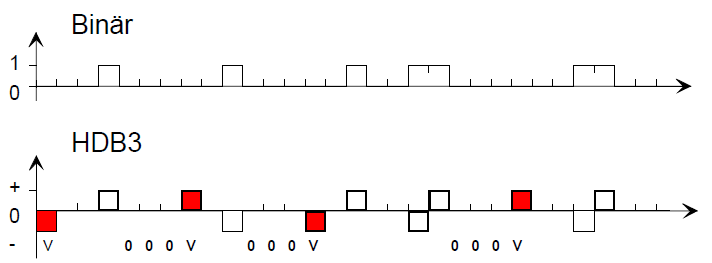
\includegraphics[height=4cm]{part1/HDB3_1}
\end{verse}
Gleichspannungsfreiheit:
\begin{itemize}
\item 4 Nullen werden nicht immer mit 000V ersetzt.
\item Ist die Anzahl Einsen (nur richtige Datenbits werden gezählt) seit
dem letzen eingefügten 000V/000B ungerade dann wird 000V verwendet,
ansonsten 000B (Polarität wechselt).\end{itemize}
\begin{verse}
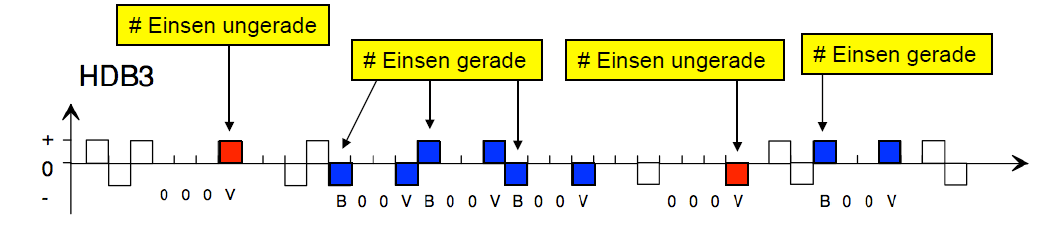
\includegraphics[height=2.5cm]{part1/HDB3_2}
\end{verse}

\section*{Frame Format}

\begin{tabular}{|c|c|}
\hline 
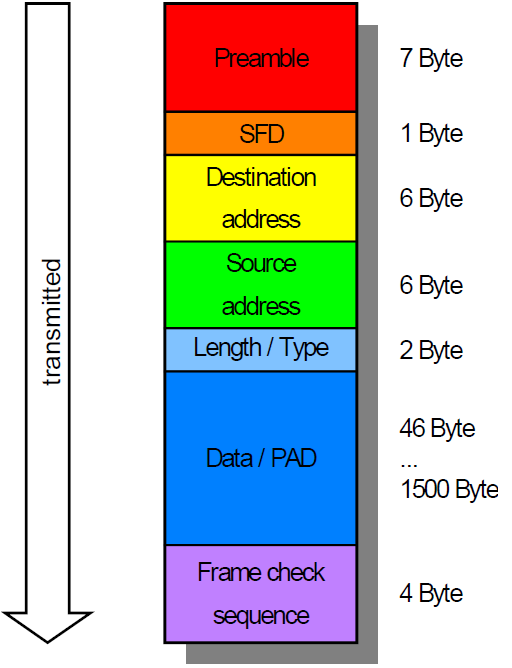
\includegraphics[width=5cm]{part1/Frame} & 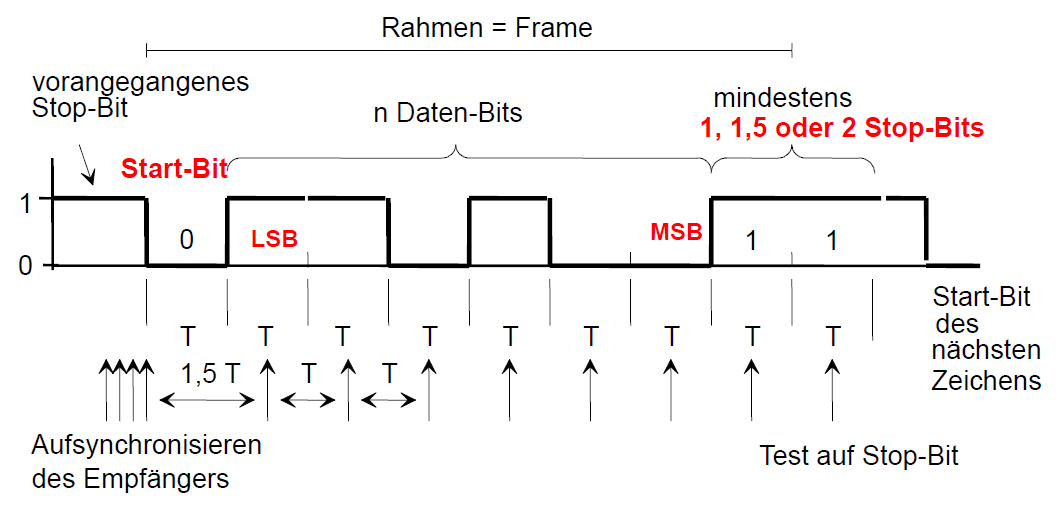
\includegraphics[height=5cm]{part1/Frameuebertragung}\tabularnewline
\hline 
\end{tabular}


\section*{Payload}
\begin{verse}
$Payload=\frac{???\, Bit/s}{8*(38+Nutzdaten)}=???Frames/s\;\Rightarrow Frames*Payload=???Bit/s$
\end{verse}
38 Bit = Präambel (8) + SFD (1) + Destination Address (6) + Source
Address (6) + Length/Type (2) + Frame Check Seq. (4) + Interframe
Gap (12) = 38
